\documentclass[12pt]{article}

\usepackage{geometry}
\usepackage[utf8]{inputenc}
\usepackage[polish]{babel}
\usepackage{polski}
\usepackage{hyperref}
\usepackage{graphicx}
\usepackage{verbatim}
\usepackage{acronym}
\usepackage{fancyhdr}
\usepackage[usenames]{color}

\hypersetup{
  linkbordercolor={1 1 1},
  urlbordercolor={1 1 1},
  colorlinks=true
}

\pagestyle{fancy}
\cfoot{}
\rfoot{\thepage}

\author{Projekt z przedmiotu Reprezentacja Wiedzy \\ \\ \textbf{Antoni Piechnik} \\ Informatyka rok IV \\ \\ prowadzący: \textbf{dr inż. Marek Gajęcki}}
\title{
Strukturyzacja słownika języka polskiego do pseudo-XML. \\
\begin{figure*}[h]
  \centerline{
    
\includegraphics[scale=1.0]{images/logo_agh.pdf}
  }
\end{figure*}
}

\begin{document}

\maketitle
\newpage
\tableofcontents
\newpage

\section{Wstęp}
\subsection{Cel Projektu}
Głownym celem projektu było stworzenie narzędzia do konwersji wypisu ze słownika
języka polskiego PWN do struktury typu XML o zadanej przez prowadzącego. Projekt
miał zaznajomić nas zarówno z formą słownika jak również problemami związanymi z
jego konwersją, na które napotkaliśmy.
\subsection{Wizja}
Projekt zaprojektowany został jako skrypt napisany w dynamicznie typowanym języku
Python, który nie tylko pozwala na sprawne przetwarzanie dużych danych, ale również
na wygodną pracę z tekstem. Skrypt składa sie z dwóch większych modułów,które
razem odpowiadają za załadowanie tekstu słownika a następnie zparsowanie go do
odpowiednich struktur.

\section{Struktura haseł słownikowych}
\subsection{Ogólne założenia}
Hasła w słowniku języka polskiego PWN z założenia powinny zawierać:
\begin{itemize}
  \item wyraz definiowany
  \item informacje dotyczące jego odmiany (niekoniecznie)
  \item definicję
  \item zdania przykładowe (niekoniecznie)
  \item przykłady zastosowań wyrazu w idiomach, nazwach specjalnych etc.
  \item pochodzenie słowa
\end{itemize}
Przykładem takiego słowa jest np.:

\begin{verbatim}
abdominalny 
1. anat. <brzuszny>
Tyfus abdominalny.
Abdominalny oddech.
2. zool. <odwłokowy>
Nogi abdominalne.
n.-łc.
\end{verbatim}

\subsection{Struktury napotkane w slowniku}
Hasła w słowniku są w zdecydowanej większości poprawnie ustrukturyzowane, jednak
istnieje wiele przypadków nie do końca poprawnych strukturalnie definicji, co 
sprawiało bardzo dużo kłopotów przy implementacji skryptu.

\section{Zadana struktura słownika}
Zadana przez prowadzącego struktura słownika w postaci konkretnych tagów pseudo-xml,
które praktycznie wystarczały do ustrukturyzowania większości z haseł zadanych w pliku
wejściowym ze słownikiem. Wyróżniono następujące tagi:

\begin{itemize}
  \item wyraz
  \item def
  \item przyklad
  \item pochodzenie
\end{itemize}

W celu rozszerzenia przykładów o te zupełnie osobno definiowane, autor projektu dodał
nowy tag sub\_def.\\

\begin{figure*}[h]
  \centerline{
    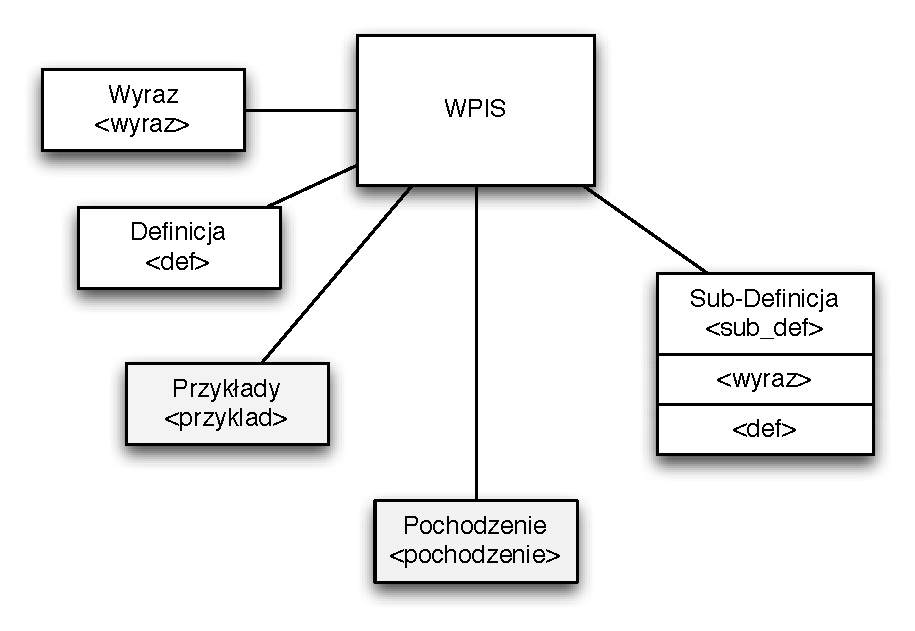
\includegraphics[scale=0.75]{images/structure.pdf}
  }
\end{figure*}


Po zastosowaniu skryptu w.wym. wpis w słowniku powinien zamienić się w następujący:

\begin{verbatim}
<wyraz>abdominalny</wyraz>
<def>(anat.) brzuszny</def>
<przyklad>Tyfus abdominalny</przyklad>
<przyklad>Abdominalny oddech</przyklad>
<pochodzenie>n.-łc.</pochodzenie>

<wyraz>abdominalny</wyraz>
<def>(zool.) odwłokowy</def>
<przyklad>Nogi abdominalne</przyklad>
<pochodzenie>n.-łc.</pochodzenie>

\end{verbatim}

\section{Struktura projektu}
\subsection{Technologie}
Skrypt został w całości napisany w języku \textbf{Python}, nie tylko ze względu na wygodę programowania
w dynamicznie typowanych językach, ale szczególnie z powodu niesłychanie potężnego narzędzia do obsługi
wyrażeń regularnych, modułów \textbf{re} oraz \textbf{string}.

\subsection{Rozwiązania}
Skrypt wczytuje dane, rozdziela poszczególne wpisy a następnie analizuje ich strukturę starając się wydzielić
odpowiednie elementy struktury (czy jest to definicja, wyraz etc.) a następnie na bazie ich położenia stara 
się przyporządkować i podzielić je w odpowiedni sposób, bazując m.in. na tym, czy jest on numerowany, czy definicja znajduje się w 
nagłówku wpisu.
Skrypt korzysta z przygotowywanych metod wykrywających czy konkretne elementy wpisu są definicją, przykładem, przykłado-definicją 
czy też opisem pochodzenia słowa. Do implementacji tychże metod posłużyły moduły wbudowane w język Python (w dużej mierze wspomniane
wcześniej \textit{re} oraz \textit{string}.

\subsection{Problemy}
Najwięcej problemów napotkano z powodu niejednoznacznej struktury podanego pliku ze słownikiem,
przez co nie można było zastosować utrwalonych schematów file-carvingu i dopasowywać skrypt do różnych
napotkanych sposobów przechowania definicji słowa w pliku słownika.

\section{Rezultaty}
Skrypt przetwarza słownik (ponad 72 tys. haseł) w niecałe 20 sekund, tworząc przy tym ponad 100 tysięcy osobnych wpisów.
W celu wydobycia informacji o jego (przynajmniej częsciowej) poprawności wprowadzono prosty system statystyk, które m.in. 
badają ile słów nie zostało przetworzonych w wyniku niekompletnego zasobu danych.

Dotychczas otrzymywaliśmy wyniki na poziomie ok 99\% przetworzonych haseł słownikowych, dalsza wersja skryptu osiągnęła
nawet wszystkie słowa bez 10 z całego słownika.

\end{document}

